\documentclass[12pt]{article}
\usepackage{amsmath}
\usepackage[rounded]{mdwtools/syntax}
\usepackage{booktabs}
\usepackage{pgf}
\usepackage{tikz}
\usetikzlibrary{arrows,automata}

\oddsidemargin 0mm
\evensidemargin 0mm
\textwidth 160mm
\textheight 200mm

\begin{document}

Final answers for the questions are shown in the boxed expressions. 

%%%%%%%%%%%%%%%%%%%%%%%%%%%%%%%%%%%%%%%%%%%%%%%%%%%%%%%%%%%%
% Question 1
%%%%%%%%%%%%%%%%%%%%%%%%%%%%%%%%%%%%%%%%%%%%%%%%%%%%%%%%%%%%
\section{}

These syntax diagrams are based off of the java documentation that was linked in the lab description.

\bigskip

Syntax for \textit{HexNumeral}:

\begin{syntdiag}
    \begin{stack} 
    	0x<HexDigits>\\
    	0X<HexDigits>
    \end{stack}
\end{syntdiag}

\bigskip

Syntax for \textit{HexDigits}:

\begin{syntdiag}
	\begin{stack}
		<HexDigit>\\
		<HexDigit>
			\begin{stack}
				<HexDigitsAndUnderscores>\\
			\end{stack}
		<HexDigit>
	\end{stack}
\end{syntdiag}

\bigskip

Syntax for \textit{HexDigit}:

\begin{syntdiag}
	\begin{stack}
		0..9\\
		a..f\\
		A..F
	\end{stack}
\end{syntdiag}

\bigskip

Syntax for \textit{HexDigitsAndUnderscores}:

\begin{syntdiag}
	\begin{stack}
		<HexDigitOrUnderscore>
		\begin{stack}
			\\
			\begin{rep}
				<HexDigitOrUnderscore>
			\end{rep}
		\end{stack}
	\end{stack}
\end{syntdiag}

\bigskip

Syntax for \textit{HexDigitOrUnderscore}:

\begin{syntdiag}
	\begin{stack}
		<HexDigit>\\
		'$\_$'
	\end{stack}
\end{syntdiag}

\bigskip

%%%%%%%%%%%%%%%%%%%%%%%%%%%%%%%%%%%%%%%%%%%%%%%%%%%%%%%%%%%%
% Question 2
%%%%%%%%%%%%%%%%%%%%%%%%%%%%%%%%%%%%%%%%%%%%%%%%%%%%%%%%%%%%
\section{}

\subsection*{(a)}

The language described by this regular expression is the set of all words that contain any number of a's and any number of b's in any order. Therefore, it is any word that is in $ \Sigma^* $, where $ \Sigma = \{a, b\}$. Formally, the language is defined as $$ \boxed{L = \{ u \mid u \in \Sigma^* \} } $$

\subsection*{(b)}

The language described by this regular expression is the set of all words that contain an even number of $b$'s. Let $ n_b(u) $ represent the number of $b$'s in the word $ u $. As well, $ a \mid b $ asserts that $a$ divides $b$, or in other words, $b$ is divisible by $a$. Let $ \Sigma = \{a, b\}$. Then, the language is formally defined as $$ \boxed{L = \{ u \mid u \in \Sigma^* \wedge 2 \mid n_b(u) \}}$$ Note: the first instance of $\mid$ in the above answer is part of the set comprehension notation. The second instance of $\mid$ refers to the notation for divisibility. 

\subsection*{(c)}

To determine the nature of this language, I will focus on subsets of the language. One subset could be derived by choosing zero instances of $a$ for the first $a^*$. This language can be described with the regular expression $$ ([ba^*c])^* $$ Now, imagine creating a subset of this language by always choosing one instance of $a$ from the remaining $a^*$. This language can be described with the regular expression $$ ([bac])^* $$ The $[bac]$ allows us to choose either $a$ or $b$ or $c$ and the $^*$ will allow us to choose one of these characters any number of times. So, if we define $ \Sigma = \{a, b, c\} $, then the regular expression $ ([bac])^* $ can generate any word that is in $\Sigma^*$. So, the subset language that I have described is formally defined as $$ \boxed{L = \{ u \mid u \in \Sigma^* \}} $$ Because the subset already contains all words in $\Sigma^*$, the original language must also be defined in the same way. This means that choosing a different number of $a$'s for each $a^*$ cannot add any new words to the language. 

%%%%%%%%%%%%%%%%%%%%%%%%%%%%%%%%%%%%%%%%%%%%%%%%%%%%%%%%%%%%
% Question 3
%%%%%%%%%%%%%%%%%%%%%%%%%%%%%%%%%%%%%%%%%%%%%%%%%%%%%%%%%%%%
\section{}

In the following examples, let $r_1$ represent the first regular expression and $r_2$ represent the second regular expression. 

\subsection*{(a)}

In $r_1$, the word $bd$ is just an instance of $bc^*d$ where zero instances of $c$ are chosen. So, this choice between $bd$ and $bc^*d$ is redundant and can be simplified to just $bc^*d$. Because the two regular expressions generate the same language, they are equivalent. $$\boxed{r_1 = r_2}$$

\subsection*{(b)}

The word $abd$ cannot be generated by $r_1$, but can be generated by $r_2$. Because the two regular expressions generate different languages, they are not equivalent. $$\boxed{r_1 \neq r_2}$$

\subsection*{(c)}

The word $b$ cannot be generated by $r_1$, but can be generated by $r_2$. Because the two regular expressions generate different languages, they are not equivalent. $$\boxed{r_1 \neq r_2}$$

%%%%%%%%%%%%%%%%%%%%%%%%%%%%%%%%%%%%%%%%%%%%%%%%%%%%%%%%%%%%
% Question 4
%%%%%%%%%%%%%%%%%%%%%%%%%%%%%%%%%%%%%%%%%%%%%%%%%%%%%%%%%%%%
\section{}

The nonterminal $A$ has the choice between two options. Choosing the production $aA$ can be used to generate one or more $a$'s. If this is not chosen immediately, then the word will contain zero $a$'s. Once the choice is made to produce $bB$, then one $b$ will be produced and any number of $b$'s or $c$'s can be generated afterwards. The regular expression for the language I have just described is given by $$ \boxed{a^*b(b \mid c)^*} $$ It is possible for the word to contain any number of $a$'s (including zero), but it must contain at least one $b$. After this first $b$, any number of $b$'s or $c$'s can follow, in any order. 

%%%%%%%%%%%%%%%%%%%%%%%%%%%%%%%%%%%%%%%%%%%%%%%%%%%%%%%%%%%%
% Question 5
%%%%%%%%%%%%%%%%%%%%%%%%%%%%%%%%%%%%%%%%%%%%%%%%%%%%%%%%%%%%
\section{}

Let $T = \{a, b, c\}$, $N = \{S, A, B, C\}$ and $P$ be a set of productions defined as $$ S \rightarrow A \mid B \mid C $$ $$ A \rightarrow aA \mid \varepsilon $$ $$ B \rightarrow bB \mid \varepsilon $$ $$ C \rightarrow abC \mid \varepsilon $$ Then, the grammar is given by $$ \boxed{G = \{T, N, P, S\}} $$

%%%%%%%%%%%%%%%%%%%%%%%%%%%%%%%%%%%%%%%%%%%%%%%%%%%%%%%%%%%%
% Question 6
%%%%%%%%%%%%%%%%%%%%%%%%%%%%%%%%%%%%%%%%%%%%%%%%%%%%%%%%%%%%
\section{}

I will convert the NFA to a DFA by using the subset construction. First, I will begin by writing out the transition table for the NFA. There are only two states and two symbols in the alphabet so there will be a total of four entries. 

\begin{table}[h]
	\begin{center}
		\begin{tabular}{|c|c|c|c|}
			\toprule
			~ & State & a & b\\
			\midrule
			$\rightarrow$ & 0 & 0, 1 & 0\\
			F: & 1 & 1 & 1\\
			\bottomrule
		\end{tabular}
	\end{center}
\end{table}

When transforming an NFA to a DFA, each state in the resulting DFA will represent a subset of the set of states of the NFA. Here, the NFA in question only has two states, which means the resulting DFA could have up to four. This is because the set of all subsets (also known as the power set) is known to have size $2^N$, where $N$ is the size of the original set. Because there are two states, the resulting DFA can have up to four ($2^2$) states. With the NFA transition table and the knowledge of the resulting DFA states, the transition table for the DFA can be constructed. The start state of the DFA will be the same as the start state of the NFA. The final states of the DFA will be any states that contain one of the final states as part of its subset. For this example, this means that any state in the resulting DFA that contains a 1 in the subset will be a final state. The transition table entries are filled in by examining the NFA and determining what states are possible to move to after an $a$ or $b$ transition in a given state.

\begin{table}[h]
	\begin{center}
		\begin{tabular}{|c|c|c|c|}
			\toprule
			~ & State & a & b\\
			\midrule
			~ & \{\} & \{\} & \{\} \\
			$\rightarrow$ & \{0\} & \{0, 1\} & \{0\} \\
			F: & \{1\} & \{1\} & \{1\} \\
			F: & \{0, 1\} & \{0, 1\} & \{0, 1\} \\
			\bottomrule
		\end{tabular}
	\end{center}
\end{table}

It is clear from the DFA transition table that the states \{\} and \{1\} cannot be reached from the start state. Therefore, they will be omitted. The resulting DFA will then have two states, called \{0\} and \{0, 1\}. The DFA will be constructed according to the specification in the transition table. Both automatons describe the language of all strings in $\Sigma^*$ that have at least one $a$. 

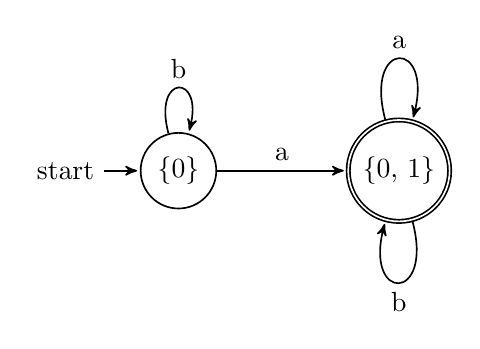
\begin{tikzpicture}[->,>=stealth',shorten >=1pt,auto,node distance=2.8cm,
                    semithick]

  \node[initial,state] (A)                    {\{0\}};
  \node[state,accepting]         (B) [right of =A] {\{0, 1\}};

  \path (A) edge [loop above] node {b} (A)
            edge              node {a} (B)
        (B) edge [loop above] node {a} (B)
            edge [loop below] node {b} (B);
\end{tikzpicture}

\end{document}